\documentclass[10pt]{article}
\usepackage[utf8]{inputenc}
\usepackage[T1]{fontenc}
\usepackage{amsmath}
\usepackage{amsfonts}
\usepackage{amssymb}
\usepackage[version=4]{mhchem}
\usepackage{stmaryrd}
\usepackage{bbold}
\usepackage{graphicx}
\usepackage[export]{adjustbox}
\graphicspath{ {./images/} }
\usepackage{caption}

\begin{document}
\captionsetup{singlelinecheck=false}
\section*{MATHEMATICS}
\section*{SECTION-A}
\begin{enumerate}
  \setcounter{enumi}{60}
  \item If the maximum distance of normal to the ellipse \(\frac{x^{2}}{4}+\frac{y^{2}}{b^{2}}=1, b<2\), from the origin is 1 , then the eccentricity of the ellipse is:\\
(1) \(\frac{1}{\sqrt{2}}\)\\
(2) \(\frac{\sqrt{3}}{2}\)\\
(3) \(\frac{1}{2}\)\\
(4) \(\frac{\sqrt{3}}{4}\)
\end{enumerate}

Official Ans. by NTA (2)\\
Allen Ans. (2)\\
Sol. Equation of normal is\\
\(2 \mathrm{x} \sec \theta-\) by \(\operatorname{cosec} \theta=4-\mathrm{b}^{2}\)\\
Distance from \((0,0)=\frac{4-b^{2}}{\sqrt{4 \sec ^{2} \theta+b^{2} \operatorname{cosec}^{2} \theta}}\)\\
Distance is maximum if\\
\(4 \sec ^{2} \theta+b^{2} \operatorname{cosec}^{2} \theta\) is minimum\\
\(\Rightarrow \tan ^{2} \theta=\frac{\mathrm{b}}{2}\)\\
\(\Rightarrow \frac{4-b^{2}}{\sqrt{4 \cdot \frac{b+2}{2}+b^{2} \cdot \frac{b+2}{b}}}=1\)\\
\(\Rightarrow 4-\mathrm{b}^{2}=\mathrm{b}+2 \Rightarrow \mathrm{~b}=1 \Rightarrow \mathrm{e}=\frac{\sqrt{3}}{2}\)\\
62. For all \(z \in C\) on the curve \(C_{1}:|z|=4\), let the locus of the point \(z+\frac{1}{z}\) be the curve \(C_{2}\). Then\\
(1) the curves \(\mathrm{C}_{1}\) and \(\mathrm{C}_{2}\) intersect at 4 points\\
(2) the curves \(\mathrm{C}_{1}\) lies inside \(\mathrm{C}_{2}\)\\
(3) the curves \(\mathrm{C}_{1}\) and \(\mathrm{C}_{2}\) intersect at 2 points\\
(4) the curves \(\mathrm{C}_{2}\) lies inside \(\mathrm{C}_{1}\)

Official Ans. by NTA (1)\\
Allen Ans. (1)

\section*{TEST PAPER WITH SOLUTION}
Sol. Let \(\mathrm{w}=\mathrm{z}+\frac{1}{\mathrm{z}}=4 \mathrm{e}^{\mathrm{i} \theta}+\frac{1}{4} \mathrm{e}^{-\mathrm{i} \theta}\)\\
\(\Rightarrow \mathrm{w}=\frac{17}{4} \cos \theta+\mathrm{i} \frac{15}{4} \sin \theta\)\\
So locus of w is ellipse \(\frac{\mathrm{x}^{2}}{\left(\frac{17}{4}\right)^{2}}+\frac{\mathrm{y}^{2}}{\left(\frac{15}{4}\right)^{2}}=1\)\\
Locus of \(z\) is circle \(x^{2}+y^{2}=16\)\\
So intersect at 4 points\\
63. A wire of length 20 m is to be cut into two pieces.

A piece of length \(\ell_{1}\) is bent to make a square of area \(A_{1}\) and the other piece of length \(\ell_{2}\) is made into a circle of area \(\mathrm{A}_{2}\). If \(2 \mathrm{~A}_{1}+3 \mathrm{~A}_{2}\) is minimum then \(\left(\pi \ell_{1}\right): \ell_{2}\) is equal to:\\
(1) \(6: 1\)\\
(2) \(3: 1\)\\
(3) \(1: 6\)\\
(4) \(4: 1\)

Official Ans. by NTA (1)\\
Allen Ans. (1)\\
Sol. \(\ell_{1}+\ell_{2}=20 \Rightarrow \frac{\mathrm{~d} \ell_{2}}{\mathrm{~d} \ell_{1}}=-1\)\\
\(\mathrm{A}_{1}=\left(\frac{\ell_{1}}{4}\right)^{2}\) and \(\mathrm{A}_{2}=\pi\left(\frac{\ell_{2}}{2 \pi}\right)^{2}\)\\
Let \(S=2 A_{1}+3 A_{2}=\frac{\ell_{1}^{2}}{8}+\frac{3 \ell_{2}^{2}}{4 \pi}\)\\
\(\frac{\mathrm{ds}}{\mathrm{d} \ell}=0 \Rightarrow \frac{2 \ell_{1}}{8}+\frac{6 \ell_{2}}{4 \pi} \cdot \frac{\mathrm{~d} \ell_{2}}{\mathrm{~d} \ell_{1}}=0\)\\
\(\Rightarrow \frac{\ell_{1}}{4}=\frac{6 \ell_{2}}{4 \pi} \Rightarrow \frac{\pi \ell_{1}}{\ell_{2}}=6\)\\
64. For the system of linear equations\\
\(x+y+z=6\)\\
\(\alpha x+\beta y+7 z=3\)\\
\(x+2 y+3 z=14\),\\
which of the following is NOT true?\\
(1) If \(\alpha=\beta=7\), then the system has no solution\\
(2) If \(\alpha=\beta\) and \(\alpha \neq 7\) then the system has a unique solution.\\
(3) There is a unique point \((\alpha, \beta)\) on the line \(x+2 y+18=0\) for which the system has infinitely many solutions\\
(4) For every point \((\alpha, \beta) \neq(7,7)\) on the line \(\mathrm{x}-2 \mathrm{y}+7=0\), the system has infinitely many solutions.

Official Ans. by NTA (4)\\
Allen Ans. (4)\\
Sol. By equation 1 and 3

\[
\begin{array}{ll} 
& \mathrm{y}=8-2 \mathrm{z} \\
\text { And } & \mathrm{x}=-2+\mathrm{z}
\end{array}
\]

Now putting in equation 2\\
\(\alpha(z-2)+\beta(-2 z+8)+7 z=3\)\\
\(\Rightarrow(\alpha-2 \beta+7) z=2 \alpha-8 \beta+3\)\\
So equations have unique solution if\\
\(\alpha-2 \beta+7 \neq 0\)\\
And equations have no solution if\\
\(\alpha-2 \beta+7=0\) and \(2 \alpha-8 \beta+3 \neq 0\)\\
And equations have infinite solution if\\
\(\alpha-2 \beta+7=0\) and \(2 \alpha-8 \beta+3=0\)\\
65. Let the shortest distance between the lines \(\mathrm{L}: \frac{\mathrm{x}-5}{-2}=\frac{\mathrm{y}-\lambda}{0}=\frac{\mathrm{z}+\lambda}{1}, \lambda \geq 0\) and \(\mathrm{L}_{1}: \mathrm{x}+1=\mathrm{y}- 1=4-z\) be \(2 \sqrt{6}\). If \((\alpha, \beta, \gamma)\) lies on \(L\), then which of the following is NOT possible?\\
(1) \(\alpha+2 \gamma=24\)\\
(2) \(2 \alpha+\gamma=7\)\\
(3) \(2 \alpha-\gamma=9\)\\
(4) \(\alpha-2 \gamma=19\)

Official Ans. by NTA (1)\\
Allen Ans. (1)

Sol. \(\quad \overrightarrow{b_{1}} \times \overrightarrow{b_{2}}=\left|\begin{array}{ccc}\hat{i} & \hat{j} & \hat{k} \\ -2 & 0 & 1 \\ 1 & 1 & -1\end{array}\right|=-\hat{i}-\hat{j}-2 \hat{k}\)\\
\(\overrightarrow{\mathrm{a}_{2}}-\overrightarrow{\mathrm{a}_{1}}=6 \hat{\mathrm{i}}+(\lambda-1) \hat{\mathrm{j}}+(-\lambda-4) \hat{\mathrm{k}}\)\\
\(2 \sqrt{6}=\left|\frac{-6-\lambda+1+2 \lambda+8}{\sqrt{1+1+4}}\right|\)\\
\(|\lambda+3|=12 \Rightarrow \lambda=9,-15\)\\
\(\alpha=-2 \mathrm{k}+5, \gamma=\mathrm{k}-\lambda\) where \(\mathrm{k} \in \mathrm{R}\)\\
\(\Rightarrow \alpha+2 \gamma=5-2 \lambda=-13,35\)\\
66. Let \(y=f(x)\) represent a parabola with focus \(\left(-\frac{1}{2}, 0\right)\) and directrix \(\mathrm{y}=-\frac{1}{2}\).

Then\\
\(\mathrm{S}=\left\{\mathrm{x} \in \mathbb{R}: \tan ^{-1}\left(\sqrt{\mathrm{f}(\mathrm{x})}+\sin ^{-1}(\sqrt{\mathrm{f}(\mathrm{x})+1})\right)=\frac{\pi}{2}\right\}:\)\\
(1) contains exactly two elements\\
(2) contains exactly one element\\
(3) is an infinite set\\
(4) is an empty set

Official Ans. by NTA (1)\\
Allen Ans. (1)\\
Sol. \(\left(\mathrm{x}+\frac{1}{2}\right)^{2}=\left(\mathrm{y}+\frac{1}{4}\right)\)\\
\(y=\left(x^{2}+x\right)\)\\
\(\tan ^{-1} \sqrt{\mathrm{x}(\mathrm{x}+1)}+\sin ^{-1} \sqrt{\mathrm{x}^{2}+\mathrm{x}+1}=\pi / 2\)\\
\(0 \leq x^{2}+x+1 \leq 1\)\\
\(x^{2}+x \leq 0\)

Also \(\mathrm{X}^{2}+\mathrm{X} \geq 0\)\\
\(\therefore \mathrm{x}^{2}+\mathrm{x}=0 \Rightarrow \mathrm{x}=0,-1\)\\
S contains 2 element.\\
67. Let \(\mathrm{A}=\left(\begin{array}{ccc}1 & 0 & 0 \\ 0 & 4 & -1 \\ 0 & 12 & -3\end{array}\right)\). Then the sum of the diagonal elements of the matrix \((\mathrm{A}+\mathrm{I})^{11}\) is equal to:\\
(1) 6144\\
(2) 4094\\
(3) 4097\\
(4) 2050

Official Ans. by NTA (3)

Allen Ans. (3)\\
Sol. \(\quad A^{2}=\left[\begin{array}{ccc}1 & 0 & 0 \\ 0 & 4 & -1 \\ 0 & 12 & -3\end{array}\right]\left[\begin{array}{ccc}1 & 0 & 0 \\ 0 & 4 & -1 \\ 0 & 12 & -3\end{array}\right]\)

\[
=\left[\begin{array}{ccc}
1 & 0 & 0 \\
0 & 4 & -1 \\
0 & 12 & -3
\end{array}\right]=A
\]

\(\Rightarrow \mathrm{A}^{3}=\mathrm{A}^{4}=\ldots \ldots=\mathrm{A}\)\\
\((\mathrm{A}+\mathrm{I})^{11}={ }^{11} \mathrm{C}_{0} \mathrm{~A}^{11}+{ }^{11} \mathrm{C}_{1} \mathrm{~A}^{10}+\ldots . .{ }^{11} \mathrm{C}_{10} \mathrm{~A}+{ }^{11} \mathrm{C}_{11} \mathrm{I}\)\\
\(=\left({ }^{11} \mathrm{C}_{0}+{ }^{11} \mathrm{C}_{1}+\ldots . .{ }^{11} \mathrm{C}_{10}\right) \mathrm{A}+\mathrm{I}\)\\
\(=\left(2^{11}-1\right) \mathrm{A}+\mathrm{I}=2047 \mathrm{~A}+\mathrm{I}\)\\
\(\therefore\) Sum of diagonal elements \(=2047(1+4-3)+3\)\\
\(=4094+3=4097\)\\
68. Let R be a relation on \(\mathrm{N} \times \mathrm{N}\) defined by \((\mathrm{a}, \mathrm{b}) \mathrm{R}\) ( \(\mathrm{c}, \mathrm{d}\) ) if and only if \(\mathrm{ad}(\mathrm{b}-\mathrm{c})=\mathrm{bc}(\mathrm{a}-\mathrm{d})\). Then R is\\
(1) symmetric but neither reflexive nor transitive\\
(2) transitive but neither reflexive nor symmetric\\
(3) reflexive and symmetric but not transitive\\
(4) symmetric and transitive but not reflexive

Official Ans. by NTA (1)\\
Allen Ans. (1)\\
Sol. \(\quad(a, b) R(c, d) \Rightarrow a d(b-c)=b c(a-d)\)\\
Symmetric:\\
\((\mathrm{c}, \mathrm{d}) \mathrm{R}(\mathrm{a}, \mathrm{b}) \Rightarrow \mathrm{cb}(\mathrm{d}-\mathrm{a})=\mathrm{da}(\mathrm{c}-\mathrm{b}) \Rightarrow\)\\
Symmetric\\
Reflexive:\\
\((\mathrm{a}, \mathrm{b}) \mathrm{R}(\mathrm{a}, \mathrm{b}) \Rightarrow \mathrm{ab}(\mathrm{b}-\mathrm{a}) \neq \mathrm{ba}(\mathrm{a}-\mathrm{b}) \Rightarrow\)\\
Not reflexive\\
Transitive: \((2,3) \mathrm{R}(3,2)\) and \((3,2) \mathrm{R}(5,30)\) but\\
\(((2,3),(5,30)) \notin \mathrm{R} \Rightarrow \quad\) Not transitive\\
69. Let\\
\(y=f(x)=\sin ^{3}\left(\frac{\pi}{3}\left(\cos \left(\frac{\pi}{3 \sqrt{2}}\left(-4 x^{3}+5 x^{2}+1\right)^{\frac{3}{2}}\right)\right)\right)\)\\
. Then, at \(\mathrm{x}=1\),\\
(1) \(2 y^{\prime}+\sqrt{3} \pi^{2} y=0\)\\
(2) \(2 y^{\prime}+3 \pi^{2} y=0\)\\
(3) \(\sqrt{2} y^{\prime}-3 \pi^{2} y=0\)\\
(4) \(y^{\prime}+3 \pi^{2} y=0\)

Official Ans. by NTA (2)\\
Allen Ans. (2)\\
Sol. \(\quad y=\sin ^{3}(\pi / 3 \cos g(x))\)\\
\(g(x)=\frac{\pi}{3 \sqrt{2}}\left(-4 x^{3}+5 x^{2}+1\right)^{3 / 2}\)\\
\(\mathrm{g}(1)=2 \pi / 3\)\\
\(y^{\prime}=3 \sin ^{2}\left(\frac{\pi}{3} \cos g(x)\right) \times \cos \left(\frac{\pi}{3} \cos g(x)\right)\)

\[
\times \frac{\pi}{3}(-\sin g(x)) g^{\prime}(x)
\]

\(y^{\prime}(1)=3 \sin ^{2}\left(-\frac{\pi}{6}\right) \cdot \cos \left(\frac{\pi}{6}\right) \cdot \frac{\pi}{3}\left(-\sin \frac{2 \pi}{3}\right) g^{\prime}(1)\)\\
\(g^{\prime}(x)=\frac{\pi}{3 \sqrt{2}}\left(-4 x^{3}+5 x^{2}+1\right)^{1 / 2}\left(-12 x^{2}+10 x\right)\)\\
\(\mathrm{g}^{\prime}(1)=\frac{\pi}{2 \sqrt{2}}(\sqrt{2})(-2)=-\pi\)\\
\(\mathrm{y}^{\prime}(1)=\frac{\not 2}{4} \cdot \frac{\sqrt{3}}{2} \cdot \frac{\pi}{\not 2}\left(\frac{-\sqrt{3}}{2}\right)(-\pi)=\frac{3 \pi^{2}}{16}\)\\
\(y(1)=\sin ^{3}(\pi / 3 \cos 2 \pi / 3)=-\frac{1}{8}\)\\
\(2 y^{\prime}(1)+3 \pi^{2} y(1)=0\)\\
70. If the sum and product of four positive consecutive terms of a G.P., are 126 and 1296, respectively, then the sum of common ratios of all such GPs is\\
(1) 7\\
(2) \(\frac{9}{2}\)\\
(3) 3\\
(4) 14

Official Ans. by NTA (1)\\
Allen Ans. (1)

Sol. a, ar, \(\mathrm{ar}^{2}, \mathrm{ar}^{3}(\mathrm{a}, \mathrm{r}>0)\)\\
\(a^{4} r^{6}=1296\)\\
\(\mathrm{a}^{2} \mathrm{r}^{3}=36\)\\
\(\mathrm{a}=\frac{6}{\mathrm{r}^{3 / 2}}\)\\
\(\mathrm{a}+\mathrm{ar}+\mathrm{ar}^{2}+\mathrm{ar}^{3}=126\)\\
\(\frac{1}{\mathrm{r}^{3 / 2}}+\frac{\mathrm{r}}{\mathrm{r}^{3 / 2}}+\frac{\mathrm{r}^{2}}{\mathrm{r}^{3 / 2}}+\frac{\mathrm{r}^{3}}{\mathrm{r}^{3 / 2}}=\frac{126}{6}=21\)\\
\(\left(\mathrm{r}^{-3 / 2}+\mathrm{r}^{3 / 2}\right)+\left(\mathrm{r}^{1 / 2}+\mathrm{r}^{-1 / 2}\right)=21\)\\
\(\mathrm{r}^{1 / 2}+\mathrm{r}^{-1 / 2}=\mathrm{A}\)\\
\(\mathrm{r}^{-3 / 2}+\mathrm{r}^{3 / 2}+3 \mathrm{~A}=\mathrm{A}^{3}\)\\
\(A^{3}-3 A+A=21\)\\
\(\mathrm{A}^{3}-2 \mathrm{~A}=21\)\\
\(\mathrm{A}=3\)\\
\(\sqrt{\mathrm{r}}+\frac{1}{\sqrt{\mathrm{r}}}=3\)\\
\(\mathrm{r}+1=3 \sqrt{\mathrm{r}}\)\\
\(\mathrm{r}^{2}+2 \mathrm{r}+1=9 \mathrm{r}\)\\
\(\mathrm{r}^{2}-7 \mathrm{r}+1=0\)\\
71. The number of real roots of the equation \(\sqrt{x^{2}-4 x+3}+\sqrt{x^{2}-9}=\sqrt{4 x^{2}-14 x+6}\), is:\\
(1) 0\\
(2) 1\\
(3) 3\\
(4) 2

Official Ans. by NTA (2)\\
Allen Ans. (2)\\
Sol. \(\sqrt{(x-1)(x-3)}+\sqrt{(x-3)(x+3)}\)\\
\(=\sqrt{4\left(x-\frac{12}{4}\right)\left(x-\frac{2}{4}\right)}\)\\
\(\Rightarrow \sqrt{\mathrm{x}-3}=0 \Rightarrow \mathrm{x}=3\) which is in domain\\
or\\
\(\sqrt{\mathrm{x}-1}+\sqrt{\mathrm{x}+3}=\sqrt{4 \mathrm{x}-2}\)\\
\(2 \sqrt{(\mathrm{x}-1)(\mathrm{x}+3)}=2 \mathrm{x}-4\)\\
\(\mathrm{x}^{2}+2 \mathrm{x}-3=\mathrm{x}^{2}-4 \mathrm{x}+4\)\\
\(6 x=7\)\\
\(x=7 / 6\) (rejected)\\
72. Let a differentiable function f satisfy \(f(x)+\int_{3}^{x} \frac{f(t)}{t} d t=\sqrt{x+1}, x \geq 3\). Then 12f(8) is equal to:\\
(1) 34\\
(2) 19\\
(3) 17\\
(4) 1

Official Ans. by NTA (3)\\
Allen Ans. (3)\\
Sol. Differentiate w.r.t. x\\
\(f^{\prime}(x)+\frac{f(x)}{x}=\frac{1}{2 \sqrt{x+1}}\)\\
I.F. \(=\mathrm{e}^{\int \frac{1}{\mathrm{x}} \mathrm{d} \mathrm{x}}=\mathrm{e}^{\ln \mathrm{x}}=\mathrm{x}\)\\
\(x f(x)=\int \frac{x}{2 \sqrt{x+1}} d x\)\\
\(\mathrm{x}+1=\mathrm{t}^{2}\)\\
\(=\int \frac{t^{2}-1}{2 t} 2 t d t\)\\
\(x f(x)=\frac{t^{3}}{3}-t+c\)\\
\(x f(x)=\frac{(x+1)^{3 / 2}}{3}-\sqrt{x+1}+c\)\\
Also putting \(\mathrm{x}=3\) in given equation\\
\(\mathrm{f}(3)+0=\sqrt{4}\)\\
\(f(3)=2\)\\
\(\Rightarrow \mathrm{C}=8-\frac{8}{3}=\frac{16}{3}\)\\
\(f(x)=\frac{\frac{(x+1)^{3 / 2}}{3}-\sqrt{x+1}+\frac{16}{3}}{x}\)\\
\(f(8)=\frac{9-3+\frac{16}{3}}{8}=\frac{34}{24}\)\\
\(\Rightarrow 12 \mathrm{f}(8)=17\)\\
73. If the domain of the function \(f(x)=\frac{[x]}{1+x^{2}}\), where \([x]\) is greatest integer \(\leq x\), is \((2,6)\), then its range is\\
(1) \(\left(\frac{5}{26}, \frac{2}{5}\right]-\left\{\frac{9}{29}, \frac{27}{109}, \frac{18}{89}, \frac{9}{53}\right\}\)\\
(2) \(\left(\frac{5}{26}, \frac{2}{5}\right]\)\\
(3) \(\left(\frac{5}{37}, \frac{2}{5}\right]-\left\{\frac{9}{29}, \frac{27}{109}, \frac{18}{89}, \frac{9}{53}\right\}\)\\
(4) \(\left(\frac{5}{37}, \frac{2}{5}\right]\)

\section*{Official Ans. by NTA (4)}
Allen Ans. (4)\\
Sol. \(f(x)=\frac{2}{1+x^{2}}\)\\
\(x \in[2,3)\)\\
\(f(x)=\frac{3}{1+x^{2}}\)\\
\(x \in[3,4)\)\\
\(f(x)=\frac{4}{1+x^{2}}\)\\
\(x \in[4,5)\)\\
\(f(x)=\frac{5}{1+x^{2}}\)\\
\(x \in[5,6)\)\\
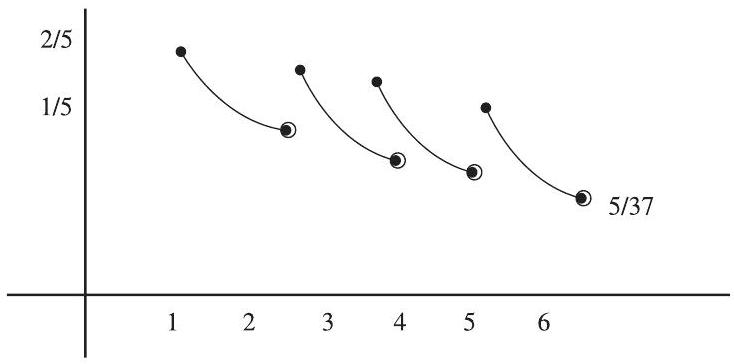
\includegraphics[max width=\textwidth, center]{2025_10_03_e8156116c478d57175e7g-05}\\
\(\left(\frac{5}{37}, \frac{2}{5}\right]\)\\
74. Let \(\vec{a}=2 \hat{i}+\hat{j}+\hat{k}\), and \(\vec{b}\) and \(\vec{c}\) be two nonzero vectors such that \(|\vec{a}+\vec{b}+\vec{c}|=|\vec{a}+\vec{b}-\vec{c}|\) and \(\overrightarrow{\mathrm{b}} \cdot \overrightarrow{\mathrm{c}}=0\). Consider the following two statement:\\
(A) \(|\overrightarrow{\mathrm{a}}+\lambda \overrightarrow{\mathrm{c}}| \geq|\overrightarrow{\mathrm{a}}|\) for all \(\lambda \in \mathbb{R}\).\\
(B) \(\overrightarrow{\mathrm{a}}\) and \(\overrightarrow{\mathrm{c}}\) are always parallel\\
(1) only (B) is correct\\
(2) neither (A) nor (B) is correct\\
(3) only (A) is correct\\
(4) both (A) and (B) are correct.

Official Ans. by NTA (3)\\
Allen Ans. (3)

Sol. \(|\vec{a}+\vec{b}+\vec{c}|^{2}=|\vec{a}+\vec{b}-\vec{c}|^{2}\)\\
\(2 \vec{a} \cdot \vec{b}+2 \vec{b} \cdot \vec{c}+2 \vec{c} \cdot \vec{a}=2 \vec{a} \cdot \vec{b}-2 \vec{b} \cdot \vec{c}-2 \vec{c} \cdot \vec{a}\)\\
\(4 \vec{a} . \vec{c}=0\)\\
B is incorrect\\
\(|\overrightarrow{\mathrm{a}}+\lambda \overrightarrow{\mathrm{c}}|^{2} \geq|\overrightarrow{\mathrm{a}}|^{2}\)\\
\(\lambda^{2} c^{2} \geq 0\)\\
True \(\forall \lambda \in \mathrm{R}\) (A) is correct.\\
75. Let \(\alpha \in(0,1)\) and \(\beta=\log _{\mathrm{e}}(1-\alpha)\). Let \(P_{n}(x)=x+\frac{x^{2}}{2}+\frac{x^{3}}{3}+\ldots . .+\frac{x^{n}}{n}, x \in(0,1)\).

Then the integral \(\int_{0}^{\alpha} \frac{\mathrm{t}^{50}}{1-\mathrm{t}} \mathrm{dt}\) is equal to\\
(1) \(\beta-\mathrm{P}_{50}(\alpha)\)\\
(2) \(-\left(\beta+\mathrm{P}_{50}(\alpha)\right)\)\\
(3) \(\mathrm{P}_{50}(\alpha)-\beta\)\\
(4) \(\beta+P_{50}(\alpha)\)

Official Ans. by NTA (2)\\
Allen Ans. (2)\\
Sol. \(\quad \int_{0}^{\alpha} \frac{\mathrm{t}^{50}-1+1}{1-\mathrm{t}}=-\int_{0}^{\alpha}\left(1+\mathrm{t}+\ldots . .+\mathrm{t}^{49}\right)+\int_{0}^{\alpha} \frac{1}{1-\mathrm{t}} \mathrm{dt}\)\\
\(=-\left(\frac{\alpha^{50}}{50}+\frac{\alpha^{49}}{49}+\ldots . .+\frac{\alpha^{1}}{1}\right)+\left(\frac{\ln (1-\mathrm{f})}{-1}\right)_{0}^{\alpha}\)\\
\(=-\mathrm{P}_{50}(\alpha)-\ln (1-\alpha)^{\prime}\)\\
\(=-\mathrm{P}_{50}(\alpha)-\beta\)\\
76. If \(\sin ^{-1} \frac{\alpha}{17}+\cos ^{-1} \frac{4}{5}-\tan ^{-1} \frac{77}{36}=0,0<\alpha<13\), then \(\sin ^{-1}(\sin \alpha)+\cos ^{-1}(\cos \alpha)\) is equal to\\
(1) \(\pi\)\\
(2) 16\\
(3) 0\\
(4) \(16-5 \pi\)

Official Ans. by NTA (1)\\
Allen Ans. (1)

Sol. \(\cos ^{-1} \frac{4}{5}=\tan ^{-1} \frac{3}{4}\)

\[
\begin{aligned}
& \therefore \sin ^{-1} \frac{\alpha}{17}=\tan ^{-1} \frac{77}{36}-\tan ^{-1} \frac{3}{4}=\tan ^{-1}\left(\frac{\frac{77}{36}-\frac{3}{4}}{1+\frac{77}{36} \cdot \frac{3}{4}}\right) \\
& \sin ^{-1} \frac{\alpha}{17}=\tan ^{-1} \frac{8}{15}=\sin ^{-1} \frac{8}{17} \\
& \Rightarrow \frac{\alpha}{17}=\frac{8}{17} \Rightarrow \alpha=8 \\
& \therefore \sin ^{-1}(\sin 8)+\cos ^{-1}(\cos 8) \\
& =3 \pi-8+8-2 \pi \\
& =\pi
\end{aligned}
\]

\begin{enumerate}
  \setcounter{enumi}{76}
  \item Let a circle \(\mathrm{C}_{1}\) be obtained on rolling the circle \(x^{2}+y^{2}-4 x-6 y+11=0\) upwards 4 units on the tangent T to it at the point \((3,2)\). Let \(\mathrm{C}_{2}\) be the image of \(\mathrm{C}_{1}\) in T . Let A and B be the centers of circles \(\mathrm{C}_{1}\) and \(\mathrm{C}_{2}\) respectively, and M and N be respectively the feet of perpendiculars drawn from \(A\) and \(B\) on the \(x\)-axis. Then the area of the trapezium AMNB is :\\
(1) \(2(2+\sqrt{2})\)\\
(2) \(4(1+\sqrt{2})\)\\
(3) \(3+2 \sqrt{2}\)\\
(4) \(2(1+\sqrt{2})\)
\end{enumerate}

Official Ans. by NTA (2)\\
Allen Ans. (2)\\
Sol. \(\quad \mathrm{C}=(2,3), \mathrm{r}=\sqrt{2}\)\\
Centre of \(\mathrm{G}=\mathrm{A}=2+4 \frac{1}{\sqrt{2}}\),\\
\(3+\frac{4}{\sqrt{2}}=(2+2 \sqrt{2}, 3+2 \sqrt{2})\)\\
\(\mathrm{A}(2+2 \sqrt{2}, 3+2 \sqrt{2})\)\\
B \((4+2 \sqrt{2}, 1+2 \sqrt{2})\)\\
\(\frac{x-(2+2 \sqrt{2})}{1}=\frac{y-(3+2 \sqrt{2})}{-1}=2\)\\
\(\therefore\) area of trapezium:\\
\(\frac{1}{2}(4+4 \sqrt{2}) 2=4(1+\sqrt{2})\)

\begin{figure}[h]
\begin{center}
  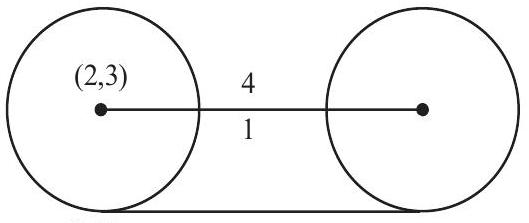
\includegraphics[width=\textwidth]{2025_10_03_e8156116c478d57175e7g-06(1)}
\captionsetup{labelformat=empty}
\caption{\((3,2)\)}
\end{center}
\end{figure}

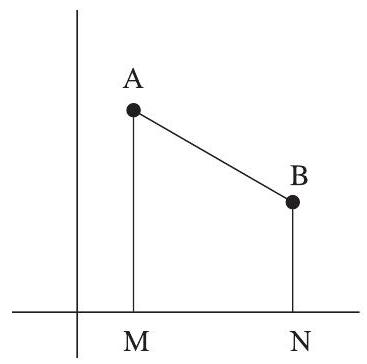
\includegraphics[max width=\textwidth, center]{2025_10_03_e8156116c478d57175e7g-06}\\
78. \((\mathrm{S} 1)(\mathrm{p} \Rightarrow \mathrm{q}) \vee(\mathrm{p} \wedge(\sim \mathrm{q}))\) is a tautology\\
\((\mathrm{S} 2)((\sim \mathrm{p}) \Rightarrow(\sim \mathrm{q})) \wedge((\sim \mathrm{p}) \vee \mathrm{q})\) is a\\
Contradiction. Then\\
(1) only (S2) is correct\\
(2) both (S1) and (S2) are correct\\
(3) both (S1) and (S2) are wrong\\
(4) only (S1) is correct

Official Ans. by NTA (2)\\
Allen Ans. (4)\\
Sol.

\begin{center}
\begin{tabular}{|c|c|c|c|c|c|}
\hline
\(\mathbf{p}\) & \(\mathbf{q}\) & \(\mathbf{p} \Rightarrow \mathbf{q}\) & \(\sim \mathbf{q}\) & \(\mathrm{p} \wedge \sim \mathrm{q}\) & \((\mathrm{p} \Rightarrow \mathrm{q}) \vee(\mathrm{p} \wedge \sim \mathrm{q})\) \\
\hline
T & T & T & F & F & T \\
\hline
T & F & F & T & T & T \\
\hline
F & T & T & F & F & T \\
\hline
F & F & T & T & F & T \\
\hline
\end{tabular}
\end{center}

\begin{center}
\begin{tabular}{|c|c|c|c|c|}
\hline
\(\sim \mathbf{p}\) & \(\sim \mathbf{q}\) & \(\sim \mathbf{p} \Rightarrow \sim \mathbf{q}\) & \(\sim \mathbf{p} \vee \mathbf{q}\) & \(((\sim \mathbf{p}) \Rightarrow(\sim \mathbf{q})) \wedge(\sim \mathbf{p}) \vee \mathbf{q})\) \\
\hline
F & F & T & T & T \\
\hline
F & T & T & F & F \\
\hline
T & F & F & T & F \\
\hline
T & T & T & T & T \\
\hline
\end{tabular}
\end{center}

\begin{enumerate}
  \setcounter{enumi}{78}
  \item The value of \(\int_{\frac{\pi}{3}}^{\frac{\pi}{2}} \frac{(2+3 \sin x)}{\sin x(1+\cos x)} d x\) is equal to\\
(1) \(\frac{7}{2}-\sqrt{3}-\log _{e} \sqrt{3}\)\\
(2) \(-2+3 \sqrt{3}+\log _{e} \sqrt{3}\)\\
(3) \(\frac{10}{3}-\sqrt{3}+\log _{e} \sqrt{3}\)\\
(4) \(\frac{10}{3}-\sqrt{3}-\log _{\mathrm{e}} \sqrt{3}\)
\end{enumerate}

Official Ans. by NTA (3)\\
Allen Ans. (3)\\
Sol. \(\quad \int_{\pi / 3}^{\pi / 2}\left(\frac{2+3 \sin \mathrm{x}}{\sin \mathrm{x}(1+\cos \mathrm{x})}\right) \mathrm{dx}=2 \int_{\pi / 3}^{\pi / 2} \frac{\mathrm{dx}}{\sin \mathrm{x}+\sin \mathrm{x} \cos \mathrm{x}}+3\)\\
\(3 \int_{\pi / 3}^{\pi / 2} \frac{\mathrm{dx}}{1+\cos \mathrm{x}}\)\\
\(\int_{\pi / 3}^{\pi / 2} \frac{\mathrm{dx}}{1+\cos \mathrm{x}}=\int_{\pi / 3}^{\pi / 2} \frac{1-\cos \mathrm{x}}{\sin ^{2} \mathrm{x}} \mathrm{dx}\)\\
\(=\int_{\pi / 3}^{\pi / 2}\left(\operatorname{cosec}^{2} \mathrm{x}-\cot \mathrm{x} \operatorname{cosec} \mathrm{x}\right) \mathrm{dx}\)\\
\(=(\operatorname{cosec} \mathrm{x}-\cot \mathrm{x}) \int_{\pi / 3}^{\pi / 2}=(1)-\left(\frac{2}{\sqrt{3}}-\frac{1}{\sqrt{3}}\right)=1-\frac{1}{\sqrt{3}}\)\\
\(\int_{\pi / 3}^{\pi / 2} \frac{d x}{\sin x(1+\cos x)}=\)\\
\(\int \frac{d x}{(2 \tan x / 2)\left(1+1-\tan ^{2} x / 2\right)}\)\\
\(=\int \frac{\left(1+\tan ^{2} x / 2\right) \sec ^{2} x / 2 d x}{2 \tan x / 2}\)\\
\(\tan \mathrm{x} / 2=\mathrm{t}\)\\
\(\sec \mathrm{x} / 2 \frac{1}{2} \mathrm{dx}=\mathrm{dt}\)\\
\(\frac{1}{2} \int\left(\frac{1+\mathrm{t}^{2}}{\mathrm{t}}\right) \mathrm{dt}=\frac{1}{2}\left[\ln \mathrm{t}+\frac{\mathrm{t}^{2}}{2}\right]_{\frac{1}{\sqrt{3}}}^{1}\)\\
\(=\frac{1}{2}\left[\left(0+\frac{1}{2}\right)-\left(\ln \frac{1}{\sqrt{3}}+\frac{1}{6}\right)\right]=\left(\frac{1}{3}+\ln \sqrt{3}\right) \frac{1}{2}\)\\
\(=\left(\frac{1}{6}+\frac{1}{2} \ell n \sqrt{3}\right)\)\\
\(2\left(\frac{1}{6}+\frac{1}{2} \ln \sqrt{3}\right)+3\left(1-\frac{1}{\sqrt{3}}\right)\)\\
\(=\frac{1}{3}+\ln \sqrt{3}+3-\sqrt{3}=\frac{10}{3}+\ln \sqrt{3}-\sqrt{3}\)\\
80. A bag contains 6 balls. Two balls are drawn from it at random and both are found to be black. The probability that the bag contains at least 5 black balls is\\
(1) \(\frac{5}{7}\)\\
(2) \(\frac{2}{7}\)\\
(3) \(\frac{3}{7}\)\\
(4) \(\frac{5}{6}\)

\section*{Official Ans. by NTA (1)}
Allen Ans. (1)\\
Sol. \(\frac{{ }^{5} \mathrm{C}_{2}+{ }^{6} \mathrm{C}_{2}}{{ }^{2} \mathrm{C}_{2}+{ }^{3} \mathrm{C}_{2}+{ }^{4} \mathrm{C}_{2}+{ }^{5} \mathrm{C}_{2}+{ }^{8} \mathrm{C}_{2}}=\frac{10+15}{1+3+6+10+15}\)\\
\(=\frac{25}{35}=\frac{5}{7}\)

\section*{SECTION-B}
\begin{enumerate}
  \setcounter{enumi}{80}
  \item Let 5 digit numbers be constructed using the digits \(0,2,3,4,7,9\) with repetition allowed, and are arranged in ascending order with serial numbers. Then the serial number of the number 42923 is\\
\(\_\_\_\_\) .
\end{enumerate}

Official Ans. by NTA (2997)

\section*{Allen Ans. (2997)}
Sol.\\
\(2+\underset{6}{++}+\underset{6}{++}+=1296\)\\
\(3++++=1296\)\\
6666\\
\(4 \underset{666}{++}+216\)\\
\(420 \underset{6}{+}+=36\)\\
\(\underline{4} \underline{2} \underline{2} \underset{6}{2}+\underset{6}{+}=36\)\\
\(423 \underset{6}{+}+=36\)\\
\(424 \underset{6}{+}+=36\)\\
\(427 \underset{6}{+}+=36\)\\
\(429 \underline{0}_{6}^{+}=6\)\\
\(42920=1\)\\
\(42922=1\)\\
\(42923=1\)\\
\(=2997\)\\
82. Let \(a_{1}, a_{2}, \ldots \ldots, a_{n}\) be in A.P. If \(a_{5}=2 a_{7}\) and \(\mathrm{a}_{11}=18\), then\\
\(12\left(\frac{1}{\sqrt{a_{10}}+\sqrt{a_{11}}}+\frac{1}{\sqrt{a_{11}}+\sqrt{a_{12}}}+\ldots . . \frac{1}{\sqrt{a_{17}}+\sqrt{a_{18}}}\right)\) is equal to \(\_\_\_\_\) .

Official Ans. by NTA (8)

Allen Ans. (8)\\
Sol. \(2 \mathrm{a}_{7}=\mathrm{a}_{5}\) (given)\\
\(2\left(a_{1}+6 d\right)=a_{1}+4 d\)\\
\(\mathrm{a}_{1}+8 \mathrm{~d}=0\)\\
\(\mathrm{a}_{1}+10 \mathrm{~d}=18\)

By (1) and (2) we get \(\mathrm{a}_{1}=-72, \mathrm{~d}=9\)\\
\(a_{18}=a_{1}+17 d=-72+153=81\)\\
\(\mathrm{a}_{10}=\mathrm{a}_{1}+9 \mathrm{~d}=9\)\\
\(12\left(\frac{\sqrt{a_{11}}-\sqrt{a_{10}}}{d}+\frac{\sqrt{a_{12}}-\sqrt{a_{11}}}{d}+\ldots \ldots \frac{\sqrt{a_{18}}-\sqrt{a_{17}}}{d}\right)\)\\
\(12\left(\frac{\sqrt{\mathrm{a}_{18}}-\sqrt{\mathrm{a}_{10}}}{\mathrm{~d}}\right)=\frac{12(9-3)}{9}=\frac{12 \times 6}{6}=8\)\\
83. Let \(\theta\) be the angle between the planes \(P_{1}=\vec{r} \cdot(\hat{i}+\hat{j}+2 \hat{k})=9\) and \(P_{2}=\vec{r} \cdot(2 \hat{i}-\hat{j}+\hat{k})=15\). Let L be the line that meets \(\mathrm{P}_{2}\) at the point ( \(4,-2,5\) ) and makes an angle \(\theta\) with the normal of \(\mathrm{P}_{2}\). If \(\alpha\) is the angle between L and \(\mathrm{P}_{2}\) then \(\left(\tan ^{2} \theta\right)\left(\cot ^{2} \alpha\right)\) is equal to \(\_\_\_\_\) .

Official Ans. by NTA (9)

Allen Ans. (9)\\
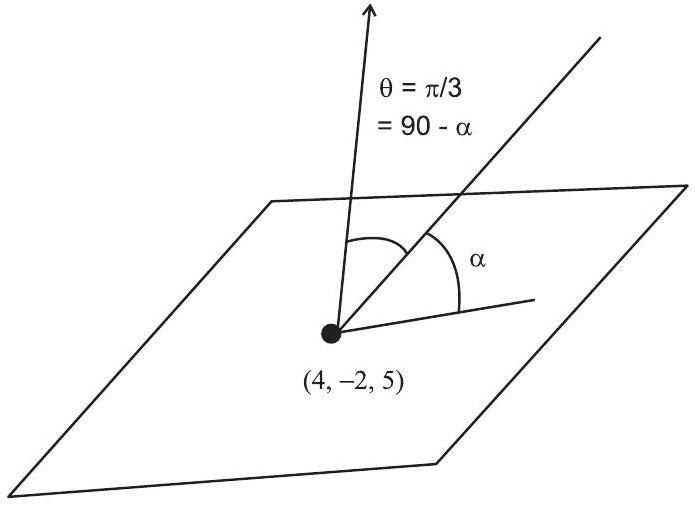
\includegraphics[max width=\textwidth, center]{2025_10_03_e8156116c478d57175e7g-08}\\
\(\cos \theta=\frac{(\hat{i}+\hat{j}+2 \hat{k}) \cdot(2 \hat{i}-\hat{j}+\hat{k})}{6}=\frac{2-1+2}{6}=\frac{1}{2}\)\\
\(\theta=\pi / 3\)\\
\(\alpha=\pi / 6\)\\
\(\left(\tan ^{2} \theta\right)\left(\cot ^{2} \alpha\right)\)\\
(3) (3) \(=9\)\\
84. Let \(\alpha>0\), be the smallest number such that the expansion of \(\left(x^{\frac{2}{3}}+\frac{2}{x^{3}}\right)^{30}\) has a term \(\beta x^{-\alpha}, \beta \in \mathbb{N}\). Then \(\alpha\) is equal to \(\_\_\_\_\) .

Official Ans. by NTA (2)\\
Allen Ans. (2)\\
Sol. \(\mathrm{T}_{\mathrm{r}+1}={ }^{30} \mathrm{C}_{\mathrm{r}}\left(\mathrm{x}^{2 / 3}\right)^{30-\mathrm{r}}\left(\frac{2}{\mathrm{x}^{3}}\right)^{\mathrm{r}}\)\\
\(={ }^{30} \mathrm{C}_{\mathrm{r}} \cdot 2^{\mathrm{r}} \cdot \mathrm{x}^{\frac{60-11 \mathrm{r}}{3}}\)\\
\(\frac{60-11 r}{3}<0 \Rightarrow 11 r>60 \Rightarrow r>\frac{60}{11} \Rightarrow r=6\)\\
\(\mathrm{T}_{7}={ }^{30} \mathrm{C}_{6} .2^{6} \mathrm{x}^{-2}\)\\
We have also observed \(\beta={ }^{30} \mathrm{C}_{6}(2)^{6}\) is a natural number.\\
\(\therefore \alpha=2\)\\
85. Let \(\vec{a}\) and \(\vec{b}\) be two vector such that \(|\vec{a}|=\sqrt{14}\), \(|\overrightarrow{\mathrm{b}}|=\sqrt{6}\) and \(|\overrightarrow{\mathrm{a}} \times \overrightarrow{\mathrm{b}}|=\sqrt{48}\). Then \((\overrightarrow{\mathrm{a}} \cdot \overrightarrow{\mathrm{b}})^{2}\) is equal to\\
\(\_\_\_\_\) .

Official Ans. by NTA (36)\\
Allen Ans. (36)

Sol. \(|\overrightarrow{\mathrm{a}}|=\sqrt{14},|\overrightarrow{\mathrm{~b}}|=\sqrt{6} \quad|\overrightarrow{\mathrm{a}} \times \overrightarrow{\mathrm{b}}|=\sqrt{48}\)\\
\(|\overrightarrow{\mathrm{a}} \times \overrightarrow{\mathrm{b}}|^{2}+|\overrightarrow{\mathrm{a}} \cdot \overrightarrow{\mathrm{b}}|^{2}=|\overrightarrow{\mathrm{a}}|^{2} \times|\overrightarrow{\mathrm{b}}|^{2}\)\\
\(\Rightarrow(\mathrm{a} \cdot \overrightarrow{\mathrm{b}})^{2}=84-48=36\)\\
86. Let the line \(L: \frac{x-1}{2}=\frac{y+1}{-1}=\frac{z-3}{1}\) intersect the plane \(2 x+y+3 z=16\) at the point \(P\). Let the point Q be the foot of perpendicular from the point \(\mathrm{R}(1,-1,-3)\) on the line L . If \(\alpha\) is the area of triangle PQR . then \(\alpha^{2}\) is equal to \(\_\_\_\_\) .

\section*{Official Ans. by NTA (180)}
\section*{Allen Ans. (180)}
Sol. Any point on \(\mathrm{L}((2 \lambda+1),(-\lambda-1),(\lambda+3))\)\\
\(2(2 \lambda+1)+(-\lambda-1)+3(\lambda+3)=16\)\\
\(6 \lambda+10=16 \Rightarrow \lambda=1\)\\
\(\therefore \mathrm{P}=(3,-2,4)\)\\
DR of \(\mathrm{QR}=\langle 2 \lambda,-\lambda, \lambda+6\rangle\)\\
DR of \(L=\langle 2,-1,1\rangle\)

\[
\begin{array}{ll}
4 \lambda+\lambda+\lambda+6=0 & 6 \lambda+6=0 \Rightarrow \lambda=-1 \\
Q=(-1,0,2) &
\end{array}
\]

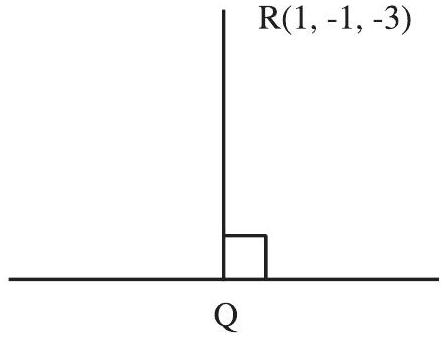
\includegraphics[max width=\textwidth, center]{2025_10_03_e8156116c478d57175e7g-09}\\
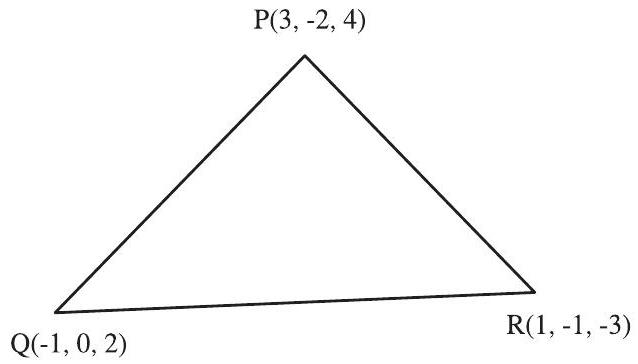
\includegraphics[max width=\textwidth, center]{2025_10_03_e8156116c478d57175e7g-09(1)}\\
\(\overrightarrow{\mathrm{QR}}=2 \hat{\mathrm{i}}-\hat{\mathrm{j}}-5 \hat{\mathrm{k}}\)\\
\(\overrightarrow{\mathrm{QP}}=4 \hat{i}-2 \hat{j}+2 \hat{k}\)\\
\(\overrightarrow{\mathrm{QR}} \times \overrightarrow{\mathrm{QP}}=\left|\begin{array}{ccc}\hat{i} & \hat{j} & \hat{k} \\ 2 & -1 & -5 \\ 4 & -2 & 2\end{array}\right|=-12 \hat{i}-24 \hat{j}\)\\
\(\alpha=\frac{1}{2} \times \sqrt{144+576} \Rightarrow \alpha^{2}=\frac{720}{4}=180\)\\
87. The remainder on dividing \(5^{99}\) by 11 is \(\_\_\_\_\) .

Official Ans. by NTA (9)\\
Allen Ans. (9)\\
Sol. \(5^{99}=5^{4} .5^{95}\)\\
\(=625\left[5^{5}\right]^{19}\)\\
\(=625[3125]^{19}\)\\
\(=625[3124+1]^{19}\)\\
\(=625[11 \mathrm{k} \times 19+1]\)\\
\(=625 \times 11 \mathrm{k} \times 19+625\)\\
\(=11 \mathrm{k}_{1}+616+9\)\\
\(=11\left(\mathrm{k}_{2}\right)+9\)\\
Remainder \(=9\)\\
88. If the variance of the frequency distribution

\begin{center}
\begin{tabular}{|c|c|c|c|c|c|c|c|}
\hline
\(\mathbf{x}_{\mathbf{i}}\) & 2 & 3 & 4 & 5 & 6 & 7 & 8 \\
\hline
Frequency \(\mathbf{f}_{\mathbf{i}}\) & 3 & 6 & 16 & \(\alpha\) & 9 & 5 & 6 \\
\hline
\end{tabular}
\end{center}

Official Ans. by NTA (5)\\
Allen Ans. (5)\\
Sol.

\begin{center}
\begin{tabular}{|l|l|l|l|l|}
\hline
 & \(\mathbf{f}_{\mathbf{i}}\) & \begin{tabular}{l}
\( \mathbf{d}_{\mathbf{i}}= \) \\
\(\mathbf{x}_{\mathbf{i}} \mathbf{- 5}\) \\
\end{tabular} & \(\mathbf{f}_{\mathbf{i}} \mathbf{d}_{\mathbf{i}}{ }^{\mathbf{2}}\) & \(\mathbf{f}_{\mathbf{i}} \mathbf{d}_{\mathbf{i}}\) \\
\hline
2 & 3 & -3 & 27 & -9 \\
\hline
3 & 6 & -2 & 24 & -12 \\
\hline
4 & 16 & -1 & 16 & -16 \\
\hline
5 & \(\alpha\) & 0 & 0 & 0 \\
\hline
6 & 9 & 1 & 9 & 9 \\
\hline
7 & 5 & 2 & 20 & 10 \\
\hline
8 & 6 & 3 & 54 & 18 \\
\hline
\end{tabular}
\end{center}

\(\sigma_{x}^{2}=\sigma_{d}^{2}=\frac{\sum f_{i} d_{i}^{2}}{\sum f_{i}}-\left(\frac{\sum f_{i} d_{i}}{\sum f_{i}}\right)^{2}\)\\
\(=\frac{150}{45+\alpha}-0=3\)\\
\(\Rightarrow 150=135+3 \alpha\)\\
\(\Rightarrow 3 \alpha=15 \Rightarrow \alpha=5\)\\
89. Let for \(x \in R\)\\
\(f(x)=\frac{x+|x|}{2}\) and \(g(x)=\left\{\begin{array}{cc}x, & x<0 \\ x^{2} & x \geq 0\end{array}\right.\).\\
Then area bounded by the curve \(\mathrm{y}=(\mathrm{fog})(\mathrm{x})\) and the lines \(\mathrm{y}=0,2 \mathrm{y}-\mathrm{x}=15\) is equal to \(\_\_\_\_\) .

Official Ans. by NTA (72)\\
Allen Ans. (72)\\
Sol. \(\quad f(x)=\frac{x+|x|}{2}=\left[\begin{array}{ll}x & x \geq 0 \\ 0 & x<0\end{array}\right.\)\\
\(g(x)=\left[\begin{array}{cc}x^{2} & x \geq 0 \\ x & x<0\end{array}\right.\)\\
\(f o g(x)=f[g(x)]=\left[\begin{array}{cc}g(x) & g(x) \geq 0 \\ 0 & g(x)<0\end{array}\right.\)\\
\(f o g(x)=\left[\begin{array}{cc}x^{2} & x \geq 0 \\ 0 & x<0\end{array}\right.\)\\
\(2 y-x=15\)\\
\(\mathrm{A}=\int_{0}^{3}\left(\frac{\mathrm{x}+15}{2}-\mathrm{x}^{2}\right) \mathrm{dx}+\frac{1}{2} \times \frac{15}{2} \times 15\)\\
\(\frac{x^{2}}{4}+\frac{15 x}{2}-\left.\frac{x^{3}}{3}\right|_{0} ^{3}+\frac{225}{4}\)\\
\(=\frac{9}{4}+\frac{45}{2}-9+\frac{225}{4}=\frac{99-36+225}{4}\)\\
\(=\frac{288}{4}=72\)\\
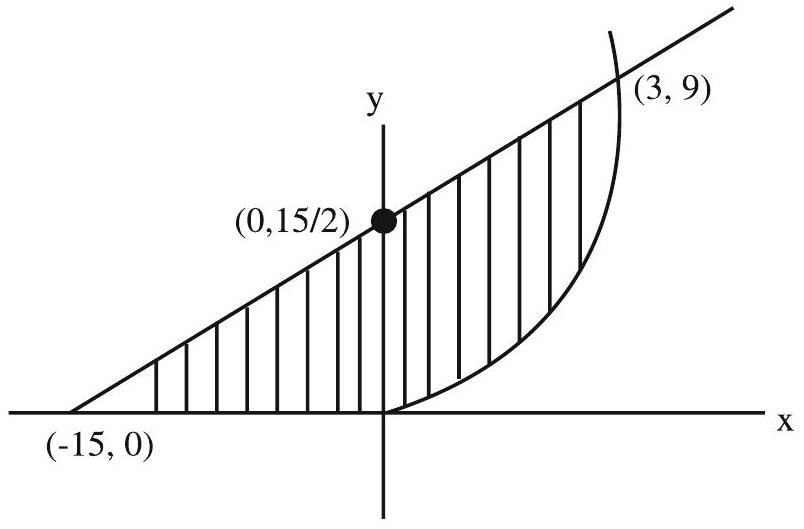
\includegraphics[max width=\textwidth, center]{2025_10_03_e8156116c478d57175e7g-10}\\
90. Number of 4-digit numbers that are less than or equal to 2800 and either divisible by 3 or by 11 , is equal to \(\_\_\_\_\) .

Official Ans. by NTA (710)

\section*{Allen Ans. (710)}
Sol. 1000-2799\\
Divisible by 3\\
\(1002+(n-1) 3=2799\)\\
\(\mathrm{n}=\mathbf{6 0 0}\)\\
Divisible by 11\\
\(1-2799 \rightarrow\left[\frac{2799}{11}\right]=[254]=254\)\\
\(1-999=\left[\frac{999}{11}\right]=90\)\\
\(1000-2799=254-90=164\)\\
Divisible by 33\\
\(1-2799 \rightarrow\left[\frac{2799}{33}\right]=84\)\\
\(1-999 \rightarrow\left[\frac{999}{33}\right]=30\)\\
\(1000-2799 \rightarrow 54\)\\
\(\therefore \mathrm{n}(3)+\mathrm{n}(11)-\mathrm{n}(33)\)\\
\(600+164-54=710\)


\end{document}